\begin{figure*}[t]
\centering
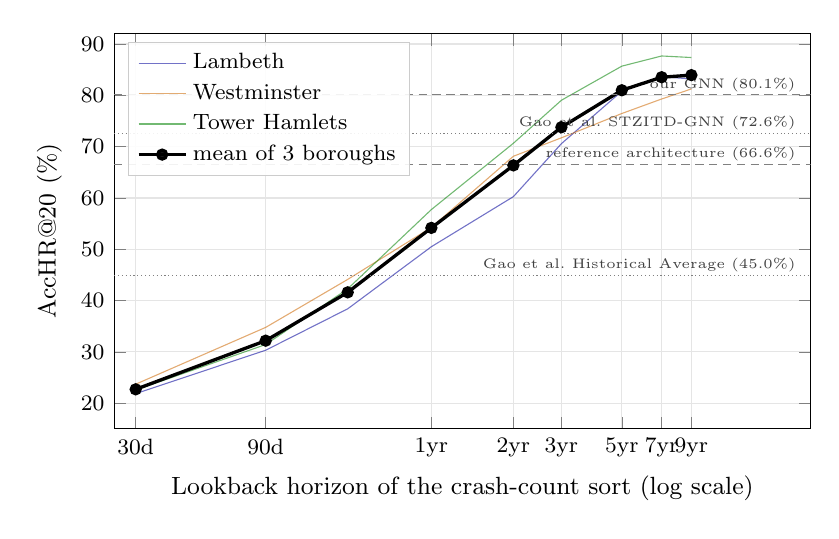
\begin{tikzpicture}
\begin{axis}[
  width=0.86\textwidth, height=6.6cm,
  xmode=log, log basis x=10,
  xlabel={Lookback horizon of the crash-count sort (log scale)},
  ylabel={AccHR@20 (\%)},
  % xmax was 3600 - only 3.9% further out than the last real data point
  % (3285) in LOG space (log10(3600/3285) = 0.039), because a log axis
  % compresses the high end far more than it looks on a linear ruler. The
  % four `anchor=east` reference-line labels below were placed at
  % x=3550, meaning "east" (their text's own right edge) sat there and
  % the text extended LEFTWARD from it - on this axis, a "tiny"-font
  % label's width corresponds to a much wider DATA range at the
  % compressed high end than the same width would at the low end, so
  % every label actually reached back well past x=3285. Three of the
  % four escaped visible collision only because their y-value sits far
  % from the curves' y-range up there (all curves are ~81-87 by 9yr);
  % "our GNN (80.1%)" at y=82.08 does not, and rendered sitting directly
  % on top of the "mean of 3 boroughs" line and its own 9yr marker
  % (confirmed 2026-09-08 by actually compiling this figure with
  % pdflatex for the first time and reading the rendered PDF page - the
  % 39 static structural checks in verify_arxiv_package.py cannot catch
  % a layout collision like this, only a real render can). Fixed at the
  % root rather than nudging one label's y-value: pushed xmax out to
  % 9000 (log10(9000/3285) = 0.437, more than 11x the old log-margin) so
  % there is a genuinely empty region to anchor labels in, and moved
  % every label's anchor to x=8600, safely inside that empty region on
  % this scale.
  xmin=25, xmax=9000, ymin=15, ymax=92,
  xtick={30,90,365,730,1095,1825,2555,3285},
  xticklabels={30d,90d,1yr,2yr,3yr,5yr,7yr,9yr},
  ytick={20,30,40,50,60,70,80,90},
  grid=major, grid style={gray!20},
  tick label style={font=\footnotesize},
  label style={font=\small},
  legend style={font=\footnotesize, at={(0.02,0.98)}, anchor=north west,
                draw=gray!40, fill=white, fill opacity=0.9, text opacity=1},
  legend cell align=left,
]
\addplot[blue!60!black, thin, opacity=0.55, mark=none] coordinates {(30,21.86) (90,30.33) (180,38.40) (365,50.50) (730,60.26) (1095,70.58) (1825,80.81) (2555,83.62) (3285,83.20)};
\addlegendentry{Lambeth}
\addplot[orange!80!black, thin, opacity=0.55, mark=none] coordinates {(30,23.71) (90,34.78) (180,44.13) (365,54.26) (730,68.13) (1095,71.72) (1825,76.46) (2555,79.29) (3285,81.25)};
\addlegendentry{Westminster}
\addplot[green!50!black, thin, opacity=0.55, mark=none] coordinates {(30,22.56) (90,31.44) (180,42.29) (365,57.74) (730,70.66) (1095,79.04) (1825,85.69) (2555,87.67) (3285,87.37)};
\addlegendentry{Tower Hamlets}
\addplot[black, very thick, mark=*, mark size=1.6pt] coordinates {(30,22.71) (90,32.19) (180,41.61) (365,54.17) (730,66.35) (1095,73.78) (1825,80.99) (2555,83.53) (3285,83.94)};
\addlegendentry{mean of 3 boroughs}
\addplot[gray, densely dotted, forget plot] coordinates {(25,44.96) (9000,44.96)};
\node[anchor=east, font=\tiny, gray!50!black] at (axis cs:8600,46.96) {Gao et al.\ Historical Average\ (45.0\%)};
\addplot[gray, densely dashed, forget plot] coordinates {(25,66.57) (9000,66.57)};
\node[anchor=east, font=\tiny, gray!50!black] at (axis cs:8600,68.57) {reference architecture\ (66.6\%)};
\addplot[gray, densely dotted, forget plot] coordinates {(25,72.60) (9000,72.60)};
\node[anchor=east, font=\tiny, gray!50!black] at (axis cs:8600,74.60) {Gao et al.\ STZITD-GNN\ (72.6\%)};
\addplot[gray, densely dashed, forget plot] coordinates {(25,80.08) (9000,80.08)};
\node[anchor=east, font=\tiny, gray!50!black] at (axis cs:8600,82.08) {our GNN\ (80.1\%)};
\end{axis}
\end{tikzpicture}
\caption{The same parameter-free crash-count sort, swept across lookback
horizons on our data and windows. The ranker spans 22.71\% to 83.94\% —
a 61.2-point range — with nothing changing but how far back it looks.
Dashed reference lines are measured on our data; dotted lines are the
reference paper's published figures on theirs, so their vertical position
is indicative rather than a controlled comparison.}
\label{fig:horizon}
\end{figure*}
